\chapter{Étude préalable}
\fancyhead[L]{\leftmark}

%====================================================
\section{Introduction}

Ce chapitre présente l'étude préalable du projet \textit{SecureRAG Hub}. Il vise à situer le projet dans son contexte scientifique, fonctionnel et technique, à formuler la problématique traitée, à préciser le périmètre de réalisation, puis à analyser les solutions existantes afin de justifier l'orientation retenue.

Le projet s'inscrit dans un contexte marqué par l'adoption rapide de l'intelligence artificielle générative dans les organisations. Les assistants conversationnels sont désormais perçus comme des leviers d'efficacité pour accéder à l'information, guider les utilisateurs et automatiser certaines interactions métiers. Toutefois, leur intégration dans un environnement professionnel soulève des enjeux majeurs : contrôle des accès, traçabilité des échanges, protection des données sensibles, gouvernance des modèles, fiabilité des réponses et maîtrise de la chaîne de déploiement.

\textit{SecureRAG Hub} répond à cette problématique en proposant une plateforme de chatbots métiers sécurisés. Le projet ne se limite pas à l'interface conversationnelle : il combine un portail web, une architecture microservices, une gouvernance par rôles, un socle Kubernetes local et une chaîne DevSecOps officielle pilotée par Jenkins. Cette orientation permet de présenter une solution démontrable, reproductible et défendable, adaptée à un Projet de Fin d'Études de niveau Master.

L'objectif de cette étude préalable est donc double. D'une part, elle clarifie les besoins et les limites du projet. D'autre part, elle montre que la valeur de la solution réside autant dans la gouvernance, la sécurité et l'industrialisation que dans la perspective d'intégration future d'un moteur d'intelligence artificielle complet.

%====================================================
\section{Cadre général du projet}

\subsection{Contexte et motivations}

\textit{SecureRAG Hub} est une plateforme unifiée de chatbots métiers sécurisés. Le projet est réalisé dans un cadre académique, au titre d'un Projet de Fin d'Études de niveau Master DSIR. Il s'appuie sur des problématiques actuelles d'architecture logicielle, de sécurité applicative, de déploiement \textit{cloud-native} et d'intégration progressive de l'intelligence artificielle.

Dans de nombreuses organisations, les utilisateurs ont besoin d'accéder rapidement à des informations dispersées : procédures RH, assistance informatique, règles internes, consignes de sécurité ou documentation technique. Les chatbots métiers constituent une réponse intéressante à ce besoin, car ils offrent une interface simple et conversationnelle. Néanmoins, un chatbot d'entreprise ne peut pas être traité comme un simple outil de génération de texte. Il doit être gouverné, audité, sécurisé et intégré dans un processus de livraison maîtrisé.

Les motivations du projet sont donc les suivantes :

\begin{itemize}
    \item proposer une interface utilisateur/administrateur claire pour gérer des chatbots métiers ;
    \item contrôler les accès grâce à une approche RBAC ;
    \item préparer l'intégration future d'une architecture RAG sans dépendre d'un LLM réel pour la soutenance ;
    \item démontrer une architecture microservices déployable localement sur Kubernetes ;
    \item industrialiser le projet avec une chaîne DevSecOps vérifiable ;
    \item produire des preuves techniques exploitables dans un mémoire et lors de la soutenance.
\end{itemize}

Cette combinaison rend le projet pertinent pour un Master DSIR, car elle relie le développement applicatif, la sécurité, l'architecture distribuée, l'automatisation CI/CD et la documentation de preuve.

\subsection{Problématique}

L'intégration de chatbots dans un environnement professionnel pose plusieurs difficultés. Les réponses doivent être adaptées au domaine métier, les utilisateurs ne doivent accéder qu'aux services autorisés, les échanges doivent pouvoir être audités et les déploiements doivent être reproductibles. À ces contraintes s'ajoute le risque spécifique aux systèmes d'intelligence artificielle générative : une réponse peut sembler cohérente tout en étant inexacte, non sourcée ou inadaptée au contexte.

La difficulté principale ne réside donc pas seulement dans la génération de réponses par un modèle d'intelligence artificielle. Elle réside dans la capacité à encadrer ces réponses, à gouverner les usages, à sécuriser les composants, à tracer les opérations et à démontrer que la plateforme déployée correspond bien à une version validée.

La problématique centrale peut être formulée ainsi :

\begin{quote}
Comment concevoir et démontrer une plateforme de chatbots métiers sécurisés, gouvernée par rôles, prête à évoluer vers le RAG, et industrialisée par une chaîne DevSecOps reproductible ?
\end{quote}

\subsection{Objectifs du projet}

Les objectifs du projet sont répartis en trois dimensions complémentaires.

Sur le plan applicatif, \textit{SecureRAG Hub} vise à fournir un portail web permettant :

\begin{itemize}
    \item l'accès différencié aux espaces utilisateur et administrateur ;
    \item la gestion des utilisateurs, des rôles et des permissions ;
    \item la gestion d'un catalogue de chatbots métiers ;
    \item la préparation des conversations et de leur historique ;
    \item la consultation d'informations de sécurité et de supervision.
\end{itemize}

Sur le plan architectural, le projet vise à :

\begin{itemize}
    \item structurer la plateforme autour de microservices ;
    \item exposer des API REST versionnées ;
    \item isoler les responsabilités entre portail, services métiers, API Gateway et composants IA ;
    \item préparer une intégration future avec un orchestrateur LLM et une base vectorielle.
\end{itemize}

Sur le plan DevSecOps, le projet vise à :

\begin{itemize}
    \item automatiser les tests, les analyses de qualité et les scans de sécurité ;
    \item utiliser Jenkins comme source officielle de CI/CD ;
    \item déployer le mode \texttt{demo} sur un cluster Kubernetes local ;
    \item produire des preuves de validation, de déploiement et de sécurité ;
    \item préparer la supply chain logicielle avec SBOM, signature, vérification et promotion par digest.
\end{itemize}

\subsection{Périmètre et limites}

Le périmètre principal couvre la réalisation d'une plateforme démontrable de chatbots métiers sécurisés. Il inclut le portail Laravel Blade, les premiers microservices métiers, les services de démonstration, le déploiement Kubernetes local, la chaîne Jenkins, les contrôles de sécurité et les documents de preuve.

Le projet ne vise pas, dans cette version, à entraîner un modèle d'intelligence artificielle, à développer un moteur RAG complet ou à garantir l'exécution d'un LLM réel en production. Ces éléments constituent des perspectives d'évolution. La version soutenable privilégie un scénario \texttt{demo} stable, dans lequel les composants IA sont représentés par des adaptateurs, des simulations ou des services contrôlés.

Cette limite est volontaire et assumée. Elle permet de distinguer clairement :

\begin{itemize}
    \item ce qui est effectivement opérationnel et validé ;
    \item ce qui est simulé afin de garantir la stabilité de la démonstration ;
    \item ce qui est prêt à être exécuté dans un environnement complet ;
    \item ce qui relève d'une extension future.
\end{itemize}

\subsection{Contraintes du projet}

Le projet est soumis à plusieurs contraintes structurantes :

\begin{itemize}
    \item maintenir un mode \texttt{demo} stable et reproductible ;
    \item éviter toute dépendance obligatoire à un modèle IA lourd ;
    \item ne jamais exposer de secrets réels dans le dépôt ;
    \item conserver une architecture lisible et modulaire ;
    \item produire des preuves techniques vérifiables ;
    \item distinguer les éléments validés des éléments dépendants de l'environnement ;
    \item rester compatible avec les outils retenus : Docker, kind, Kubernetes, Kustomize, Jenkins, Semgrep, Gitleaks, Trivy, Syft, Cosign et Kyverno.
\end{itemize}

Ces contraintes orientent fortement la conception. Elles expliquent notamment le choix d'un mode \texttt{demo} officiel, la séparation entre services applicatifs et composants IA, ainsi que l'importance accordée aux runbooks et aux artefacts de validation.

%====================================================
\section{Cadre académique et parties prenantes}

\subsection{Cadre académique du projet}

Le projet est réalisé dans un cadre académique. Il ne dépend pas, dans l'état actuel du mémoire, d'un organisme d'accueil dont les informations seraient officiellement documentées. Afin d'éviter toute approximation, cette section présente donc le cadre fonctionnel et pédagogique du projet plutôt qu'une description institutionnelle non vérifiée.

Si un organisme d'accueil doit être ajouté dans la version finale, il conviendra d'y intégrer uniquement des informations confirmées : nom de l'organisme, domaine d'activité, missions, service d'affectation, encadrants, coordonnées et contexte exact du besoin.

\subsection{Parties prenantes fonctionnelles}

La plateforme cible plusieurs profils d'acteurs :

\begin{itemize}
    \item les utilisateurs métiers, qui interagissent avec les chatbots selon leur domaine ;
    \item les administrateurs plateforme, responsables de la configuration générale ;
    \item les administrateurs sécurité, chargés de suivre les incidents et les journaux ;
    \item l'équipe DevSecOps, responsable des pipelines, des scans, des déploiements et des preuves ;
    \item le jury de soutenance, qui évalue la cohérence fonctionnelle, technique et méthodologique du projet.
\end{itemize}

Cette identification des parties prenantes permet de clarifier les priorités : le projet doit être utilisable, gouverné, démontrable et documenté.

\subsection{Organisation fonctionnelle simplifiée}

L'organisation fonctionnelle du projet peut être représentée ainsi :

\begin{figure}[htbp]
    \centering
    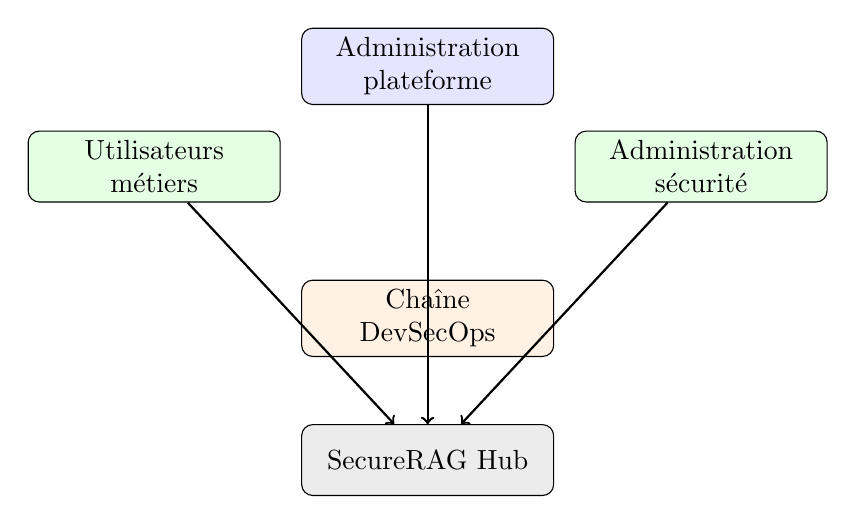
\begin{tikzpicture}[
        node distance=1.8cm,
        every node/.style={draw, rounded corners, align=center, minimum width=3.2cm, minimum height=0.9cm}
    ]
        \node[fill=blue!10] (admin) {Administration\\plateforme};
        \node[fill=green!10, below left of=admin, xshift=-2.2cm] (users) {Utilisateurs\\métiers};
        \node[fill=green!10, below right of=admin, xshift=2.2cm] (security) {Administration\\sécurité};
        \node[fill=orange!10, below of=admin, yshift=-1.4cm] (devsecops) {Chaîne\\DevSecOps};
        \node[fill=gray!15, below of=devsecops] (platform) {SecureRAG Hub};

        \draw[->, thick] (admin) -- (platform);
        \draw[->, thick] (users) -- (platform);
        \draw[->, thick] (security) -- (platform);
        \draw[->, thick] (devsecops) -- (platform);
    \end{tikzpicture}
    \caption{Organisation fonctionnelle simplifiée autour de SecureRAG Hub}
    \label{fig:organigramme_fonctionnel_securerag}
\end{figure}

%====================================================
\section{Concepts clés du projet}

Cette section présente uniquement les notions nécessaires à la compréhension de \textit{SecureRAG Hub}. L'objectif n'est pas de proposer un cours général sur l'intelligence artificielle ou Kubernetes, mais de définir les concepts directement mobilisés par le projet.

\subsection{Chatbot métier et plateforme sécurisée}

Un chatbot est un programme capable d'interagir avec un utilisateur à travers une interface conversationnelle. Un chatbot métier se distingue d'un chatbot généraliste par son rattachement à un domaine précis : ressources humaines, support informatique, sécurité, documentation interne ou assistance administrative.

Dans \textit{SecureRAG Hub}, le chatbot métier n'est pas seulement un canal de discussion. Il est associé à un domaine fonctionnel, à un niveau de sensibilité, à des rôles autorisés, à une configuration de prompt et à des règles de traçabilité. Cette approche permet de traiter le chatbot comme une ressource gouvernée plutôt que comme une simple interface d'IA.

\subsection{Intelligence artificielle, apprentissage automatique et IA générative}

L'intelligence artificielle désigne un ensemble de techniques permettant à un système informatique d'accomplir des tâches qui requièrent habituellement des capacités humaines : classification, prédiction, reconnaissance, analyse ou génération de contenu. L'apprentissage automatique en constitue une branche majeure : le système apprend à partir de données au lieu d'être entièrement programmé par des règles explicites.

Trois familles d'apprentissage sont particulièrement utiles à situer. L'apprentissage supervisé utilise des exemples annotés pour apprendre à prédire une catégorie ou une valeur. L'apprentissage non supervisé cherche des structures dans des données non annotées, par exemple à travers le clustering. L'apprentissage profond repose sur des réseaux de neurones multicouches et constitue l'une des bases des modèles de langage modernes \cite{russell_norvig_ai,goodfellow_deep_learning}.

L'intelligence artificielle générative est la branche qui produit du contenu à partir d'une requête : texte, résumé, code, réponse conversationnelle ou aide à la décision. Les modèles de langage de grande taille, ou LLM, font partie de cette famille. Ils peuvent générer des réponses cohérentes, mais ils peuvent également produire des réponses erronées ou non vérifiées. Ce risque, souvent appelé hallucination, impose une gouvernance stricte dans un contexte professionnel \cite{bommasani_foundation_models,ji_hallucination_survey}.

Dans le projet, l'IA est traitée comme une capacité architecturale préparée, non comme un moteur complet déjà industrialisé. Le scénario officiel repose sur le mode \texttt{demo}, afin de démontrer la plateforme sans dépendre d'un LLM réel.

\subsection{RAG et base documentaire}

La génération augmentée par récupération, ou RAG, combine une recherche documentaire avec une génération de réponse. Le système recherche d'abord des documents pertinents dans une base contrôlée, puis transmet ces éléments au modèle de langage pour produire une réponse contextualisée \cite{lewis_rag_2020}.

Cette approche est importante dans une plateforme métier, car elle réduit la dépendance aux connaissances générales du modèle et favorise des réponses fondées sur des sources internes. Elle nécessite généralement une base documentaire, des embeddings, une base vectorielle et un orchestrateur chargé de préparer le contexte.

Dans \textit{SecureRAG Hub}, la logique RAG complète n'est pas développée dans la première version. La plateforme prépare cependant son intégration future grâce à une architecture séparant portail, API Gateway, microservices, orchestrateur LLM et service de connaissance.

\subsection{RBAC et gouvernance des accès}

Le RBAC, ou contrôle d'accès basé sur les rôles, consiste à associer des permissions à des rôles, puis des rôles aux utilisateurs. Cette approche convient à une plateforme multi-profils, dans laquelle un administrateur plateforme, un administrateur sécurité, un utilisateur RH et un utilisateur IT ne doivent pas disposer des mêmes droits.

Dans \textit{SecureRAG Hub}, les rôles structurants sont notamment \texttt{super-admin}, \texttt{admin-plateforme}, \texttt{admin-securite}, \texttt{user-rh} et \texttt{user-it}. Cette séparation permet de gouverner l'accès aux utilisateurs, aux chatbots, aux conversations, aux incidents et aux preuves DevSecOps.

\subsection{Architecture microservices et API REST}

Une architecture microservices découpe une application en services autonomes, chacun responsable d'un périmètre fonctionnel. Cette organisation favorise la maintenabilité, l'évolutivité et la séparation des responsabilités \cite{newman_microservices}.

Dans le projet, les microservices couvrent notamment les utilisateurs et le RBAC, le catalogue de chatbots, les conversations, l'audit et les services de démonstration. Les échanges sont structurés autour d'API REST versionnées, par exemple sous le préfixe \texttt{/api/v1}. Cette convention facilite la stabilisation des contrats entre le portail Blade et les services métiers.

\subsection{Kubernetes, conteneurisation et déploiement local}

La conteneurisation permet d'embarquer une application et ses dépendances dans une image exécutable. Docker est utilisé pour construire et lancer ces images. Kubernetes permet ensuite d'orchestrer les conteneurs, de gérer les déploiements, les services, les volumes, les politiques réseau et certaines capacités de résilience.

Pour rester démontrable localement, \textit{SecureRAG Hub} utilise \texttt{kind}, c'est-à-dire Kubernetes in Docker. Cette solution permet de créer un cluster Kubernetes local reproductible. Les manifests sont organisés avec Kustomize afin de séparer une base commune et des overlays, notamment \texttt{dev} et \texttt{demo} \cite{kubernetes_docs,kind_docs,kustomize_docs}.

\subsection{DevSecOps et supply chain logicielle}

DevSecOps désigne l'intégration continue de la sécurité dans le cycle DevOps. La sécurité n'est plus un contrôle final, mais un ensemble de vérifications intégrées dès le code source, puis dans les tests, les scans, la construction des images, la signature, le déploiement et l'admission Kubernetes.

Dans \textit{SecureRAG Hub}, Jenkins constitue la source officielle de CI/CD. Les contrôles incluent Ruff pour la qualité Python, Semgrep pour l'analyse statique, Gitleaks pour la détection de secrets, Trivy pour l'analyse de vulnérabilités, Syft pour la génération de SBOM et Cosign pour la signature et la vérification des images. La promotion par digest permet de déployer l'image effectivement validée, plutôt qu'une image reconstruite ou référencée uniquement par un tag.

Cette chaîne peut être résumée ainsi :

\begin{center}
\texttt{code -> tests -> scans -> build -> SBOM -> sign -> verify -> promote -> deploy -> validate}
\end{center}

La mise en place complète de cette supply chain avancée dépend de l'environnement d'exécution, notamment du registre local, des clés Cosign, de Syft, de Docker et du cluster Kubernetes. Le mémoire doit donc distinguer les étapes validées, les étapes prêtes à être rejouées et les étapes dépendantes de l'environnement.

\subsection{Sécurité Kubernetes}

La sécurité Kubernetes repose sur plusieurs mécanismes complémentaires. Les \textit{NetworkPolicies} restreignent les communications entre pods. Les \textit{ResourceQuotas} et \textit{LimitRanges} encadrent l'utilisation des ressources. Les \textit{PodDisruptionBudgets} améliorent la disponibilité lors des perturbations. Les \textit{HorizontalPodAutoscalers} préparent l'élasticité, à condition que \texttt{metrics-server} fournisse les métriques nécessaires.

Kyverno permet d'ajouter des politiques d'admission Kubernetes. En mode \texttt{Audit}, les ressources non conformes sont signalées sans être bloquées. En mode \texttt{Enforce}, elles peuvent être refusées. Pour une soutenance, il est important de présenter cette distinction avec rigueur afin de ne pas confondre une politique prête à être appliquée avec une politique réellement active en blocage.

\subsection{Technologies non retenues dans la version actuelle}

Certaines technologies, comme la blockchain, peuvent être pertinentes pour des cas de traçabilité inter-organisationnelle. Toutefois, elles ne sont pas nécessaires dans cette version du projet. Les besoins de preuve sont couverts de manière plus directe par les journaux d'audit, les digests OCI, les signatures d'images, les rapports de validation et les artefacts Jenkins.

Ce choix évite d'alourdir l'architecture avec une technologie qui ne répond pas à un besoin central du périmètre actuel.

%====================================================
\section{Analyse et critique de l'existant}

\subsection{Critères d'analyse}

L'analyse de l'existant s'appuie sur les critères suivants : qualité de l'expérience conversationnelle, gouvernance des accès, intégration aux données internes, maîtrise de l'infrastructure, capacité de déploiement local, traçabilité, sécurité et visibilité sur la chaîne DevSecOps.

Ces critères permettent de comparer \textit{SecureRAG Hub} aux solutions commerciales et techniques du marché, sans prétendre rivaliser avec elles sur la puissance des modèles ou la maturité produit.

\subsection{Solutions commerciales orientées entreprise}

Des solutions comme ChatGPT Enterprise, Microsoft Copilot Studio, Google Vertex AI Agent Builder, Amazon Q Business ou IBM watsonx Assistant proposent déjà des assistants IA destinés aux organisations. Elles se distinguent par leur maturité, leur qualité d'expérience utilisateur, leurs connecteurs, leurs capacités d'administration et leur intégration à des écosystèmes cloud ou bureautiques \cite{openai_chatgpt_enterprise,microsoft_copilot_studio,google_vertex_ai_agent_builder,aws_q_business,ibm_watsonx_assistant}.

Leurs points forts sont importants : elles permettent une adoption rapide, offrent des modèles puissants, bénéficient d'infrastructures robustes et réduisent l'effort de développement initial. Elles sont particulièrement adaptées aux entreprises qui souhaitent consommer un service managé plutôt que construire une plateforme complète.

Leurs limites apparaissent dans le cadre de ce projet. Elles dépendent fortement d'un fournisseur, masquent une grande partie de la chaîne technique interne et ne permettent pas toujours de démontrer localement le cycle complet : construction d'images, génération de SBOM, signature Cosign, vérification, promotion par digest, déploiement Kubernetes et collecte de preuves.

Par rapport à ces solutions, \textit{SecureRAG Hub} se positionne différemment. Il ne cherche pas à proposer le meilleur modèle conversationnel. Il cherche à démontrer une architecture maîtrisée, sécurisée, reproductible et explicable devant un jury.

\subsection{Frameworks et plateformes techniques}

Des solutions comme Rasa, Botpress, LangChain ou LangGraph répondent à des besoins plus techniques. Rasa et Botpress facilitent la construction d'assistants conversationnels personnalisés. LangChain et LangGraph permettent de concevoir des workflows LLM, des chaînes RAG et des orchestrations plus avancées \cite{rasa_docs,botpress_docs,langchain_docs,langgraph_docs}.

Leur principal atout est la flexibilité. Elles conviennent aux équipes qui veulent construire des agents ou des assistants sur mesure. Elles offrent davantage de contrôle qu'une solution SaaS entièrement managée.

Cependant, ces outils ne fournissent pas à eux seuls une plateforme complète de gouvernance, de sécurité, de RBAC, de déploiement Kubernetes, de signature d'images et de preuve DevSecOps. Ils constituent plutôt des briques pouvant être intégrées dans une architecture plus large.

\textit{SecureRAG Hub} peut donc être compris comme une plateforme d'intégration autour de ces briques potentielles. Dans une version future, LangChain ou LangGraph pourraient enrichir l'orchestration IA, tandis que Rasa ou Botpress pourraient inspirer certains mécanismes conversationnels. Dans la version actuelle, ils restent des perspectives et non des dépendances centrales.

\subsection{Positionnement de SecureRAG Hub}

L'analyse montre que les solutions existantes sont généralement fortes sur l'un des axes suivants : puissance conversationnelle, intégration cloud, productivité de création d'agents ou flexibilité de développement. En revanche, elles mettent moins l'accent sur une démonstration locale complète associant portail métier, microservices, RBAC, Kubernetes, Jenkins, supply chain et preuves.

Le positionnement de \textit{SecureRAG Hub} est donc le suivant :

\begin{itemize}
    \item offrir une plateforme académique complète plutôt qu'un simple chatbot ;
    \item rendre explicite la gouvernance des utilisateurs, des rôles et des chatbots ;
    \item démontrer une architecture \textit{cloud-native} reproductible localement ;
    \item intégrer la sécurité dans la chaîne de livraison ;
    \item produire des preuves techniques exploitables en soutenance ;
    \item préparer l'intégration future du RAG sans la présenter comme déjà pleinement réalisée.
\end{itemize}

Cette position est défendable car elle évite une comparaison directe avec les grandes plateformes commerciales sur leur terrain principal. La valeur du projet réside dans la cohérence entre application métier, architecture distribuée, sécurité et industrialisation.

%====================================================
\section{Solution proposée}

\subsection{Principe général}

La solution proposée, \textit{SecureRAG Hub}, est organisée en plusieurs couches. Le portail Laravel Blade constitue la surface utilisateur. Les microservices portent la logique métier. L'API Gateway prépare un point d'entrée technique. Kubernetes exécute les composants conteneurisés. Jenkins orchestre la CI/CD et les validations de sécurité.

\begin{figure}[htbp]
    \centering
    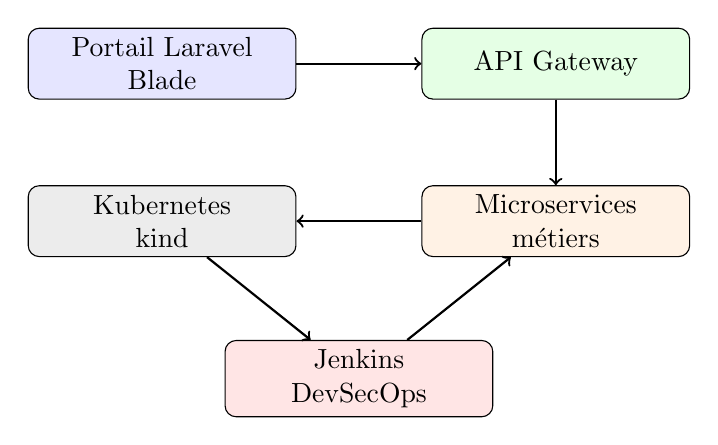
\begin{tikzpicture}[
        node distance=1.9cm,
        every node/.style={draw, rounded corners, align=center, minimum width=3.4cm, minimum height=0.9cm}
    ]
        \node[fill=blue!10] (portal) at (0,0) {Portail Laravel\\Blade};
        \node[fill=green!10] (gateway) at (5,0) {API Gateway};
        \node[fill=orange!10] (services) at (5,-2) {Microservices\\métiers};
        \node[fill=gray!15] (k8s) at (0,-2) {Kubernetes\\kind};
        \node[fill=red!10] (devsecops) at (2.5,-4) {Jenkins\\DevSecOps};

        \draw[->, thick] (portal) -- (gateway);
        \draw[->, thick] (gateway) -- (services);
        \draw[->, thick] (services) -- (k8s);
        \draw[->, thick] (k8s) -- (devsecops);
        \draw[->, thick] (devsecops) -- (services);
    \end{tikzpicture}
    \caption{Vue simplifiée de l'architecture SecureRAG Hub}
    \label{fig:vue_simplifiee_securerag}
\end{figure}

\subsection{Fonctionnalités prévues}

La plateforme regroupe les fonctionnalités suivantes :

\begin{itemize}
    \item espace utilisateur pour accéder aux chatbots autorisés ;
    \item espace administrateur pour gérer utilisateurs, rôles et chatbots ;
    \item gestion du catalogue de chatbots métiers ;
    \item préparation des conversations et de l'historique ;
    \item supervision des incidents et des preuves DevSecOps ;
    \item API REST destinées à connecter progressivement les écrans Blade aux services persistants.
\end{itemize}

\subsection{Choix techniques}

Laravel Blade est retenu pour le portail afin de réduire la complexité frontend et de conserver une interface claire, maintenable et adaptée au périmètre académique. Vue.js et Inertia ne sont pas utilisés dans cette version.

Laravel est également retenu pour les microservices métiers persistants, car il fournit un cadre robuste pour les migrations, les modèles Eloquent, les Form Requests, les policies, les seeders et les tests. Des services FastAPI sont conservés pour stabiliser le scénario de démonstration.

Docker, \texttt{kind}, Kubernetes et Kustomize assurent la reproductibilité du déploiement. Jenkins constitue la source officielle de CI/CD. Les outils Semgrep, Gitleaks, Trivy, Syft, Cosign et Kyverno renforcent la dimension DevSecOps.

\subsection{Justification du mode demo}

Le mode \texttt{demo} est retenu comme scénario officiel de soutenance. Ce choix garantit une démonstration stable, contrôlée et indépendante d'un modèle IA lourd. Il permet également de présenter clairement l'état réel du projet : le socle DevSecOps et Kubernetes est démontrable, les capacités IA sont préparées architecturalement, et l'intégration RAG complète reste une perspective.

Ce positionnement est important face au jury. Il évite de promettre un système IA complet alors que la valeur principale du projet est la construction d'une plateforme sécurisée, industrialisée et prête à évoluer.

%====================================================
\section{Langage et méthodologie de conception}

\subsection{Méthodologie Scrum}

Le projet adopte une démarche agile inspirée de Scrum. Ce choix est justifié par la diversité des composants à réaliser : portail web, API, microservices, Kubernetes, sécurité, CI/CD, documentation et preuves de soutenance. Une approche strictement séquentielle aurait été peu adaptée, car plusieurs contraintes ont évolué au cours du projet, notamment la stabilité du mode \texttt{demo}, l'accès à GitHub depuis Jenkins ou l'exécution complète de la supply chain.

Scrum repose sur trois principes utiles dans ce contexte : transparence, inspection et adaptation. La transparence consiste à documenter l'état réel du projet. L'inspection consiste à valider chaque incrément par des tests, des scans ou des commandes reproductibles. L'adaptation consiste à ajuster les priorités lorsque l'environnement impose des limites.

Chaque sprint devait produire un livrable vérifiable : un écran, une API, un script, un manifeste Kubernetes, un rapport de scan, un support pack ou une section du mémoire. Cette logique a permis d'éviter une progression purement théorique.

\begin{table}[htbp]
    \centering
    \begin{tabular}{|p{2.2cm}|p{5.2cm}|p{6.2cm}|}
        \hline
        \textbf{Sprint} & \textbf{Objectif principal} & \textbf{Livrables représentatifs} \\
        \hline
        Sprint 1 & Cadrage et architecture initiale & Périmètre, scénario \texttt{demo}, structure du dépôt \\
        \hline
        Sprint 2 & Socle applicatif et conteneurisation & Services de démonstration, Dockerfiles, endpoints de santé \\
        \hline
        Sprint 3 & Kubernetes local & Cluster \texttt{kind}, registry locale, Kustomize, overlays \\
        \hline
        Sprint 4 & Sécurité et CI de base & Tests, couverture, Ruff, Semgrep, Gitleaks, Trivy \\
        \hline
        Sprint 5 & Jenkins et campagne finale & Jobs CI/CD, fallback \texttt{/workspace}, campagne \texttt{demo/dry-run} \\
        \hline
        Sprint 6 & Portail Blade & Page d'accueil, tableaux de bord, vues utilisateur/administrateur \\
        \hline
        Sprint 7 & Microservices métiers & Services Laravel, RBAC, catalogue chatbots, tests \\
        \hline
        Sprint 8 & Preuves et mémoire & Support pack, runbooks, validation finale, alignement documentaire \\
        \hline
    \end{tabular}
    \caption{Application progressive de Scrum au projet SecureRAG Hub}
    \label{tab:sprints_securerag}
\end{table}

\subsection{Choix du langage de conception}

Le langage principal de conception retenu est UML, car il permet de représenter les besoins fonctionnels, la structure métier, les interactions et le déploiement. UML est adapté à un mémoire académique, car il fournit une notation standard et compréhensible pour décrire un système logiciel complexe.

Les diagrammes les plus pertinents pour \textit{SecureRAG Hub} sont les suivants :

\begin{itemize}
    \item le diagramme de cas d'utilisation, pour identifier les acteurs et les fonctionnalités ;
    \item le diagramme de classes, pour représenter utilisateurs, rôles, permissions, chatbots, conversations et incidents ;
    \item le diagramme de séquence, pour décrire les échanges entre portail, API Gateway et microservices ;
    \item le diagramme de composants, pour montrer la séparation entre portail, services, API Gateway et infrastructure ;
    \item le diagramme de déploiement, pour expliquer l'exécution sur Docker, kind et Kubernetes.
\end{itemize}

En complément, une représentation de type C4 peut être utilisée afin de clarifier les niveaux d'architecture : contexte, conteneurs, composants et déploiement. Pour la partie DevSecOps, des diagrammes de pipeline permettent de représenter la chaîne :

\begin{center}
\texttt{push Git -> Jenkins CI -> tests -> scans -> build -> sign -> verify -> deploy}
\end{center}

Cette combinaison entre UML, C4 et diagrammes DevSecOps rend la conception plus lisible et relie les choix logiciels à leur exécution opérationnelle.

%====================================================
\section{Bénéfices attendus et perspectives}

\subsection{Bénéfices attendus}

Les bénéfices attendus de \textit{SecureRAG Hub} sont les suivants :

\begin{itemize}
    \item fournir une plateforme structurée pour gérer des chatbots métiers ;
    \item sécuriser l'accès aux fonctionnalités par rôles et permissions ;
    \item démontrer une architecture microservices déployable localement ;
    \item intégrer la sécurité dans la chaîne de livraison logicielle ;
    \item produire des preuves exploitables en soutenance ;
    \item préparer une évolution vers un moteur RAG réel.
\end{itemize}

\subsection{Perspectives d'évolution}

Les perspectives principales concernent :

\begin{itemize}
    \item la connexion complète des écrans Blade aux microservices Laravel persistants ;
    \item l'achèvement des services de conversation et d'audit ;
    \item la formalisation des contrats OpenAPI ;
    \item l'intégration d'un moteur RAG réel ;
    \item l'amélioration de l'observabilité ;
    \item l'exécution complète de la supply chain en mode \texttt{execute} ;
    \item le passage progressif des policies Kyverno du mode \texttt{Audit} vers le mode \texttt{Enforce}.
\end{itemize}

Ces perspectives sont cohérentes avec l'état réel du projet. Elles prolongent la plateforme sans remettre en cause le scénario \texttt{demo} validé.

%====================================================
\section{Conclusion}

Cette étude préalable a permis de définir le cadre du projet \textit{SecureRAG Hub}, d'en formuler la problématique, d'en préciser le périmètre et d'en analyser le positionnement par rapport aux solutions existantes. Elle montre que le projet ne doit pas être évalué comme un simple chatbot, mais comme une plateforme complète associant gouvernance métier, architecture microservices, sécurité, Kubernetes et DevSecOps.

Le chapitre a également clarifié une distinction essentielle : la plateforme est prête à évoluer vers une intégration IA/RAG plus complète, mais le scénario officiel de soutenance repose sur un mode \texttt{demo} maîtrisé. Cette décision renforce la fiabilité de la démonstration et évite de promettre un niveau d'IA non encore industrialisé.

Le chapitre suivant pourra donc approfondir la conception de la solution, en détaillant les acteurs, les cas d'utilisation, les modèles de données, l'architecture logicielle et les choix de déploiement retenus.
